\section{$z$-Transform}
\begin{frame}{Introduction}
    \begin{itemize}
        \item We developed the Laplace transform as a generalization of the continuous-time Fourier transform.
        \item In this lecture, we introduce the corresponding generalization of the discrete-time Fourier transform.
        \item The resulting transform is referred to as the $z$-transform.
    \end{itemize}
\end{frame}


\begin{frame}{$z$-Transform Motivation}
    \begin{itemize}
        \item The discrete-time Fourier transform developed out of choosing complex exponentials as basic building blocks for signals because they are eigenfunctions of discrete-time LTI systems.
        \item A more general class of eigenfunctions consists of signals of the form $z^n$, where $z$ is a general complex number. A representation of discrete-time signals with these more general exponentials leads to the $z$-transform.
    \end{itemize}
\end{frame}

\begin{frame}{Relationship between the $z$-Transform and the Discrete-Time Fourier Transform}
    \begin{itemize}
        \item We saw that the Laplace transform is a generalization of the continuous-time Fourier transform.
        \item A close relationship exists between the $z$-transform and the discrete-time Fourier transform.
        \item For $z = e^{j\omega}$ or, equivalently, for the magnitude of $z$ equal to unity, the $z$-transform reduces to the Fourier transform.
        \item More generally, the $z$-transform can be viewed as the Fourier transform of an exponentially weighted sequence.
        \item Because of this, the $z$-transform may converge for a given sequence even if the Fourier transform does not: the $z$-transform offers the possibility of transform analysis for a broader class of signals and systems.
    \end{itemize}
\end{frame}

\begin{frame}{The Region of Convergence (ROC)}
    \begin{itemize}
        \item The $z$-transform of a signal too has associated with it both  a range of values of $z$, referred to as the region of convergence (ROC), for which this expression is valid.
        \item Two different sequences can have $z$-transforms with identical algebraic expressions such that their $z$-transforms differ only in the ROC.
        \item Consequently, the ROC is an important part of the specification of the $z$-transform.
    \end{itemize}
\end{frame}


\begin{frame}{$z$-Plane}
    \begin{itemize}
        \item $z$-transforms of the form of a ratio of polynomials in $z^{-1}$ are described by poles and zeros in the complex plane, referred to as the $z$-plane.
        \item The circle of radius 1, concentric with the origin in the $z$-plane, is  referred to as the \alert{unit circle}.
        \item Since this circle corresponds to the magnitude of $z$ equal to unity, it is the contour in the $z$-plane on which the $z$-transform reduces to the Fourier transform.
        \item In contrast, for continuous time it is the imaginary axis in the $s$-plane on which the Laplace transform reduces to the Fourier transform.
        \item If the sequence is known to be right-sided, for example, then the ROC must be the portion of the $z$-plane outside the circle bounded by the outermost pole.
    \end{itemize}
\end{frame}

\subsection{The $z$-Transform}

\begin{frame}{Recall: Discrete-Time Fourier Transform}
    \begin{align*}
        x[n] &= \frac{1}{2\pi}\int_{2\pi}X(e^{j\omega})e^{j\omega n}d\omega\\
        X(e^{j\omega}) &= \sum_{-\infty}^{+\infty}x[n]e^{-j\omega n}\\
    \end{align*}
    LTI systems: impulse response $h(t)$:
    \begin{equation*}
        \begin{matrix}
            e^{j\omega n} & \rightarrow & \quad H(e^{j\omega})e^{j\omega n} \\
            && \negthickspace\updownarrow{\mathcal{F}}\\
            && \negthickspace h[n]\\
        \end{matrix}
    \end{equation*}
\end{frame}


\begin{frame}{$z$-Transform: Eigenfunction Property}
    \begin{align*}
        z^{n} &\rightarrow \sum_{k=-\infty}^{+\infty}h[k]z^{n-k}\\
        z^{n} &\rightarrow z^{n}\sum_{k=-\infty}^{+\infty}h[k]z^{-k}\\
        z &= re^{j\omega}\\
        z^{n}   &\rightarrow H(z) z^{n}\\
        H(z) &= \sum_{n=-\infty}^{+\infty}h[n]z^{-n}
    \end{align*}
\end{frame}


\begin{frame}{$z$-Transform}
    \begin{align*}
        X(z) &= \sum_{n=-\infty}^{+\infty}x[n]z^{-n}\\
        x[n] &\xleftrightarrow{\mathcal{Z}} X(z)
    \end{align*}
\end{frame}


\begin{frame}{$z$-Transform and Fourier Transform Relationship}
    \begin{align*}
        X(\omega) &= \sum_{n=-\infty}^{+\infty}x[n]e^{-j\omega n}\\
        X(z) &= \sum_{n=-\infty}^{+\infty}x[n]z^{-n}\\
        z &= re^{j\omega}\\
        \left.X(z)\right|_{z=e^{j\omega}} &= \mathcal{F}\left\{ x[n]\right\}
    \end{align*}
    New notation:
    \begin{equation*}
        \mathcal{F}\left\{ x[n]\right\} = X(e^{j\omega})
    \end{equation*}
\end{frame}

\begin{frame}{$z$-Transform: Convergence Comparison}
    \begin{align*}
        \left.X(z)\right|_{z=e^{j\omega}} &= X(e^{j\omega})\\
        X(z) &= \sum_{n=-\infty}^{+\infty}x[n]z^{-n}\\
        X(re^{j\omega}) &= \sum_{n=-\infty}^{+\infty}x[n]\left(re^{j\omega}\right)^{-n}\\
        &= \sum_{n=-\infty}^{+\infty}x[n]r^{-n}re^{-j\omega n}\\
        X(z) &= \mathcal{F}\left\{ x[n]r^{-n}\right\}
    \end{align*}
    \uncover<2->
    {
        ZT may converge when FT does not.
    }
\end{frame}

\begin{frame}[t]{}
    \begin{example}
        Find the ZT of
        $
            x[n] = a^nu[n].
        $
    \end{example}

    \mode<beamer>
    {
        \begin{solution}
        \end{solution}
            \begin{align*}
                %X(e^{j\omega}) &= \frac{1}{1-ae^{-j\omega}}, \quad |a|<1\\
                %\pause
                X(z) &= \sum_{n=-\infty}^{+\infty}x[n]z^{-n}\\
                &= \sum{n=-\infty}^{+\infty}a^nz^{-n}u[n]\\
                X(s) &= \frac{1}{1-az^{-1}}, \quad |az^{-1}|< 1\\
            \end{align*}\pause
            \begin{equation*}
                a^nu[n] \xleftrightarrow{\mathcal{Z}}   \frac{1}{1-az^{-1}}, \quad |z|> |a|
            \end{equation*}
    }
\end{frame}





\begin{frame}[t]{}
    \begin{example}
        Find the ZT of
        \begin{equation*}
            x[n] = -a^nu[-n-1].
        \end{equation*}
    \end{example}
    \pause
    \mode<beamer>
    {
        \begin{solution}\end{solution}
            \begin{align*}
                X(z) &= \sum_{n=-\infty}^{+\infty}x[n]z^{-n}\\
                &= -\sum_{n=-\infty}^{+\infty}a^nz^{-n}u[-n-1]\\
                X(s) &= \frac{1}{1-az^{-1}}, \quad |az^{-1}|>1\\
            \end{align*}
            \pause
            \begin{equation*}
                -a^nu[-n-1] \xleftrightarrow{\mathcal{Z}}   \frac{1}{1-az^{-1}}, \quad |z|< |a|
            \end{equation*}

    }
\end{frame}


\begin{frame}{$z$-Plane and the Unit Circle}
    \mode<beamer>
    {
        \begin{center}
            \begin{tikzpicture}[scale=0.8]
    \def\pole{++(135:0.1) -- ++(-45:0.2) ++(135:0.1) -- ++(45:0.1) -- ++(-135:0.2) +(45:0.1)}
    \def\zero{circle (0.1)}
    \draw (-3, 0) -- (1,0) node[anchor=west] {$\mathrm{Re}$};
    \draw (0, -3) -- (0,3) node[anchor=south] {$\mathrm{Im}$};
    \path [pattern color=pink, pattern=north east lines] (-1, 0) ++(0,3) rectangle ++(2, -6);
    \draw (-1,0) node[anchor=north] {\scriptsize$-1$} \pole (-2, 0)  node[anchor=north] {\scriptsize$-2$}\pole (-1.5, 0) node[anchor=north] {\scriptsize $ -\frac{3}{2}$}\zero;

\end{tikzpicture} 
        \end{center}
    }
\end{frame}

\begin{frame}{Pole-Zero Plot for a Right-Handed Sequence}
    \begin{equation*}
        a^nu[n] \xleftrightarrow{\mathcal{Z}}   \frac{1}{1-az^{-1}} = \frac{z}{z-a}, \quad |z|> |a|
    \end{equation*}
    \mode<beamer>
    {
        \begin{center}
            \begin{tikzpicture}[scale=0.6]
    \def\pole{++(135:0.1) -- ++(-45:0.2) ++(135:0.1) -- ++(45:0.1) -- ++(-135:0.2) +(45:0.1)}
    \def\zero{circle (0.1)}
    \draw (-3, 0) -- (1,0) node[anchor=west] {$\mathrm{Re}$};
    \draw (0, -3) -- (0,3) node[anchor=south] {$\mathrm{Im}$};
    \path [pattern color=pink, pattern=north east lines] (-1, 0) ++(0,3) rectangle ++(2, -6);
    \draw (-1,0)  \pole (-2, 0)  \pole ;
\end{tikzpicture}
        \end{center}
    }
\end{frame}


\begin{frame}{Pole-Zero Plot for a Left-Handed Sequence}
    \begin{equation*}
        -a^nu[-n-1] \xleftrightarrow{\mathcal{Z}}   \frac{1}{1-az^{-1}} = \frac{z}{z-a},  \quad |z|< |a|
    \end{equation*}
    \mode<beamer>
    {
        \begin{center}
            %\usetikzlibrary{patterns}
\begin{tikzpicture}[scale=0.8]
    \def\pole{++(135:0.1) -- ++(-45:0.2) ++(135:0.1) -- ++(45:0.1) -- ++(-135:0.2) +(45:0.1)}
    \def\zero{circle (0.1)}
    	%\begin{scope}
     		%\path [pattern color=pink, pattern=north east lines] (-3, -3)  rectangle (3, 3);
     		\draw [dashed, pattern color=pink, pattern=north east lines] (0,0) circle (1.5);
	%\end{scope}

    \draw (-3, 0) -- (3,0) node[anchor=west] {\scriptsize $\mathrm{Re}$};
    \draw (0, -3) -- (0,3) node[anchor=south] {\scriptsize $\mathrm{Im}$};
    %\pause
    \draw[thick, magenta] (0,0) circle (2);
    \draw [latex-] (0,0) ++(135:2) -- ++(135:0.5) node [anchor=south east] {\scriptsize Unit circle};
    \node at (2, 0) [anchor=north west] {\scriptsize $1$};

    \node at (2, 1) [anchor=west] {\scriptsize $z$-plane};
    \draw (1.5, 0) node[anchor=north east] {$a$} \pole (0,0) \zero;

\end{tikzpicture} 
        \end{center}
    }
\end{frame}

\begin{frame}{First-Order Difference Equation}
    \begin{equation*}
        y[n] - ay[n-1] = x[n]
    \end{equation*}
    \pause
    \mode<beamer>
    {
        \begin{equation*}
            Y(z) - az^{-1}Y(z) = X(z)
        \end{equation*}
        \pause
        \begin{equation*}
            Y(z) = \frac{1}{1 - az^{-1}} X(z)
        \end{equation*}
        \pause
        \begin{equation*}
            H(z) = \frac{1}{1 - az^{-1}}
        \end{equation*}
        Causality: \pause $|z|>|a|$
        \pause
        \begin{equation*}
            h[n] = a^nu[n]
        \end{equation*}
    }
\end{frame}


\begin{frame}{Pole-Zero Plot for a DT First-Order System}
    This illustrates the determination of the Fourier transform form the pole-zero plot.
    \begin{equation*}
        H(z) = \frac{z}{z-a}, \quad |z| >|a|.
    \end{equation*}
    \mode<beamer>
    {
        \begin{center}
            %\usetikzlibrary{patterns}
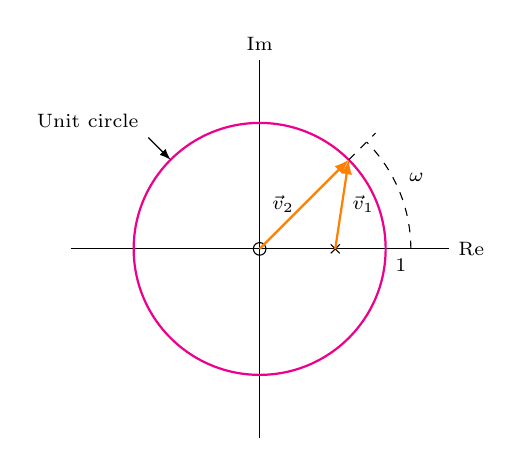
\begin{tikzpicture}[scale=0.8]
    \def\pole{++(135:0.1) -- ++(-45:0.2) ++(135:0.1) -- ++(45:0.1) -- ++(-135:0.2) +(45:0.1)}
    \def\zero{circle (0.1)}

    \draw (-3, 0) -- (3,0) node[anchor=west] {\scriptsize $\mathrm{Re}$};
    \draw (0, -3) -- (0,3) node[anchor=south] {\scriptsize $\mathrm{Im}$};
    %\pause
    \draw[thick, magenta] (0,0) circle (2);
    \draw [latex-] (0,0) ++(135:2) -- ++(135:0.5) node [anchor=south east] {\scriptsize Unit circle};
    \node at (2, 0) [anchor=north west] {\scriptsize $1$};

    %\node at (2, 1) [anchor=west] {\scriptsize $z$-plane};
    \coordinate (p1) at (0:1.2);
    %\coordinate (p2) at (-60:1.5);    
    \coordinate (o) at (0,0);
    \coordinate (a) at (45:2);
    \draw (p1) node[anchor=north east] {} \pole;
     %\draw (p2) node[anchor=north east] {} \pole;
    \draw (0,0) \zero;
    %\draw (0,0) circle (0.07);
    
    
    \draw[dashed] (o) -- (p1);
    %\draw[dashed] (o) -- (p2);    
    \draw[dashed]  (45:2) -- ++(45:0.6);
    \draw[-latex, thick, orange] (p1) -- (a) node [midway, black, anchor=west] {\scriptsize $\vec{v}_1$};
  \draw[-latex, thick, orange] (o) -- (a) node [midway, black, anchor=east] {\scriptsize $\vec{v}_2$};       
  %\draw[-latex, thick, orange] (p2) -- (a);         
  
  \draw[dashed] (2.4,0) arc (0:45:2.4)  node [midway, anchor=south west] {\scriptsize $\omega$};    ;
 % \draw (0.6,0) arc (0:-60:0.6);  
  %\node at (20:0.8) {\scriptsize $\theta$};
  %\node at (-20:0.8) {\scriptsize $\theta$};  
   %\node at (a) [anchor=south west] {\scriptsize $\Omega=\theta$};    

\end{tikzpicture} 
        \end{center}
    }
\end{frame}

\begin{frame}{Second-Order Difference Equation}
    \begin{equation*}
        y[n] + 2r\cos\theta y[n-1] + r^2y[n-2]= x[n]
    \end{equation*}
    \pause
    \mode<beamer>
    {
        \begin{equation*}
            Y(z)\left[1+2r\cos\theta z^{-1} + r^2z^{-2}\right] = X(z)
        \end{equation*}
        \pause
        \begin{equation*}
            Y(z) = \frac{1}{1+2r\cos\theta z^{-1} + r^2z^{-2}} X(z)
        \end{equation*}
        \pause
        \begin{equation*}
            H(z) = \frac{1}{1+2r\cos\theta z^{-1} + r^2z^{-2}}
        \end{equation*}
        $\cos\theta < 1 \Rightarrow$  complex poles\\
        Poles are at
        \pause
        \begin{equation*}
            re^{\pm j \theta}
        \end{equation*}
    }
\end{frame}

\begin{frame}{Pole-Zero Plot for a DT Under-Damped Second-Order System}
    This illustrates the determination of the Fourier transform form the pole-zero plot.
    \begin{equation*}
        H(z) = \frac{1}{1-(2r\cos\theta)z^{-1} + r^2z^{-2}}, \quad |z| >|a|.
    \end{equation*}
    \mode<beamer>
    {
        \begin{center}
            \begin{tikzpicture}[scale=0.6]
    \def\pole{++(135:0.1) -- ++(-45:0.2) ++(135:0.1) -- ++(45:0.1) -- ++(-135:0.2) +(45:0.1)}
    \def\zero{circle (0.1)}
    \draw (-3, 0) -- (1,0) node[anchor=west] {$\mathrm{Re}$};
    \draw (0, -3) -- (0,3) node[anchor=south] {$\mathrm{Im}$};
    \path [pattern color=pink, pattern=north east lines] (-2, 0) ++(0,3) rectangle ++(-1, -6);
    \draw (-1,0)  \pole (-2, 0)  \pole ;
\end{tikzpicture}
        \end{center}
    }
\end{frame}




\begin{frame}{Properties of the ROC of the $z$-Transform}
    \begin{itemize}
      \item The ROC does not contain poles
      \item The ROC of $X(z)$ consists of a ring in the $z$-plane centered about the origin
      \item $\mathcal{F}\{x[n]\}$ converges $\Leftrightarrow$ ROC includes the unit circle in the $z$-plane
      \item $x[n]$ finite duration $\Rightarrow$ ROC is entire $z$-plane with the possible exception of $z = 0$ or $z = \infty$
    \end{itemize}
\end{frame}

\begin{frame}{Properties of the ROC for a Right-Sided Sequence}
    \begin{itemize}
      \item $x[n]$ right-sided and $|z| = r_0$ is in ROC $\Rightarrow$ all finite values of $z$ for which $|z| > r_0$ are in ROC.
      \item $x[n]$ right-sided and $X(z)$ rational $\Rightarrow$ ROC is outside the outermost pole.
    \end{itemize}
\end{frame}

\begin{frame}{Properties of the ROC for a Left-Sided and for a Two-Sided Sequence}
    \begin{itemize}
      \item $x[n]$ left-sided and $|z| = r_0$ is in ROC $\Rightarrow$ all  values of $z$ for which $0 < |z| < r_0$ will also be in ROC.
      \item $x[n]$ left-sided and $X(z)$ rational $\Rightarrow$ ROC is inside  the innermost pole.
      \item $x[n]$ two-sided and $|z| = r_0$ is in ROC $\Rightarrow$ ROC is a ring in the  $z$-plane which includes the circle $|z|= r_0$.
    \end{itemize}
\end{frame}

\begin{frame}
    \begin{example}
        Show the choices of the ROC for
        \begin{equation*}
            X(z) = \frac{z}{\left(z - \frac{1}{3}\right)\left(z-2\right)}.
        \end{equation*}
    \end{example}
\end{frame}

\begin{frame}{ROC If the Sequence Is Right-Sided.}
    \begin{equation*}
        X(z) = \frac{z}{\left(z - \frac{1}{3}\right)\left(z-2\right)}.
    \end{equation*}
    \mode<beamer>
    {
        %\begin{solution}
        \begin{center}
            \begin{tikzpicture}[scale=0.6]
    \def\pole{++(135:0.1) -- ++(-45:0.2) ++(135:0.1) -- ++(45:0.1) -- ++(-135:0.2) +(45:0.1)}
    \def\zero{circle (0.1)}
    \draw (-3, 0) -- (1,0) node[anchor=west] {$\mathrm{Re}$};
    \draw (0, -3) -- (0,3) node[anchor=south] {$\mathrm{Im}$};
    \path [pattern color=pink, pattern=north east lines] (-1, 0) ++(0,3) rectangle ++(2, -6);
    \draw (-1,0) node[anchor=north] {\scriptsize$-1$} \pole (-2, 0)  node[anchor=north] {\scriptsize$-2$} \pole;

\end{tikzpicture} 
        \end{center}
        %\end{solution}
    }
\end{frame}

\begin{frame}{ROC If the Sequence Is Left-Sided.}
    \begin{equation*}
        X(z) = \frac{z}{\left(z - \frac{1}{3}\right)\left(z-2\right)}.
    \end{equation*}
    \mode<beamer>
    {
        %\begin{solution}
        \begin{center}
            \usetikzlibrary{patterns}
\begin{tikzpicture}[scale=0.8]
    \def\pole{++(135:0.1) -- ++(-45:0.2) ++(135:0.1) -- ++(45:0.1) -- ++(-135:0.2) +(45:0.1)}
    \def\zero{circle (0.1)}
    	\begin{scope}
     		%\path [pattern color=pink, pattern=north east lines] (-3, -3)  rectangle (3, 3);
     		\draw [dashed, pattern color=pink, pattern=north east lines] (0,0) circle (2);
	\end{scope}

    \draw (-3, 0) -- (3,0) node[anchor=west] {\scriptsize $\mathrm{Re}$};
    \draw (0, -3) -- (0,3) node[anchor=south] {\scriptsize $\mathrm{Im}$};
    %\pause
    \draw[thick, magenta] (0,0) circle (1);
    \draw [latex-] (0,0) ++(135:1) -- ++(135:1.5) node [anchor=south east] {\scriptsize Unit circle};

    \node at (2, 1) [anchor=west] {\scriptsize $z$-plane};
    \draw (2, 0) node[anchor=north west] {$2$} \pole;
    \draw (1/3, 0) node[anchor=north ] {$\frac{1}{3}$} \pole;
	\draw    (0,0) \zero;
\end{tikzpicture} 
        \end{center}
        %\end{solution}
    }
\end{frame}

\begin{frame}{ROC If the Sequence Is Two-Sided.}
    \begin{equation*}
        X(z) = \frac{z}{\left(z - \frac{1}{3}\right)\left(z-2\right)}.
    \end{equation*}
    \mode<beamer>
    {
        %\begin{solution}\end{solution}
        \begin{center}
            \begin{tikzpicture}[scale=0.6]
    \def\pole{++(135:0.1) -- ++(-45:0.2) ++(135:0.1) -- ++(45:0.1) -- ++(-135:0.2) +(45:0.1)}
    \def\zero{circle (0.1)}
    \draw (-3, 0) -- (1,0) node[anchor=west] {$\mathrm{Re}$};
    \draw (0, -3) -- (0,3) node[anchor=south] {$\mathrm{Im}$};
    \path [pattern color=pink, pattern=north east lines] (-1, 0) ++(0,3) rectangle ++(2, -6);
    \draw[dashed] (-2, -3) -- (-2, 3);
    \path [pattern color=orange, pattern=north west lines] (-2, 0) ++(0,3) rectangle ++(1, -6);
    \draw (-2,0) node[anchor=north] {\scriptsize$-2$} (-1,0) node[anchor=north] {\scriptsize$-1$};

\end{tikzpicture} 
        \end{center}

    }
\end{frame}

\begin{frame}{Inverse $z$-Transform}
    \begin{align*}
        X(z) &= \mathcal{F}\left\{x[n]r^{-n}\right\}\\
        x[n]r^{-n} &= \mathcal{F}^{-1}\left\{X(z)\right\}\\
        &= \frac{1}{2\pi}\int_{2\pi}X(re^{j\omega}) e^{-j\omega n}d\omega\\
        x[n] &= \frac{1}{2\pi}\int_{2\pi}X(re^{j\omega})\left(re^{j\omega}\right)^nd\omega\\
        z &= re^{j\omega}, \qquad dz = jre^{j\omega}d\omega\\
        x[n] &= \frac{1}{2\pi j} \oint X(z)z^{n-1}dz
    \end{align*}
\end{frame}


\begin{frame}
    \begin{example}
        \begin{equation*}
            X(z) = \frac{z}{\left(z-\frac{1}{3}\right)(z-2)}, \quad |z|>2.
        \end{equation*}
    \end{example}
    \pause
    \mode<beamer>
    {
        %\begin{solution}\end{solution}
            \begin{align*}
                X(z) &= \frac{z}{\left(z-\frac{1}{3}\right)(z-2)}, \quad |z|>2,\\
                &= \frac{z^{-1}}{\left(1-\frac{1}{3}z^{-1}\right)(1-2z^{-1})}, \quad |z|>2,\\
                &= \frac{-\frac{3}{5}}{\left(1-\frac{1}{3}z^{-1}\right)} + \frac{-\frac{3}{5}}{(1-2z^{-1})}, \quad |z|>2.\\
                \pause
                x[n] &=  -\frac{3}{5} \left(\frac{1}{3}\right)^nu[n] + \frac{3}{5} (2)^n u[n].\\
            \end{align*}

    }
\end{frame}




\subsection{$z$-Transform properties}
\begin{frame}{Recall: $z$-Transform}
    \begin{align*}
        X(z) &= \sum_{n=-\infty}^{+\infty}x[n]z^{-n}\\
        x[n] &= \frac{1}{2\pi j}\ointctrclockwise X(z)z^{-n}dz\\
        \left.X(z)\right|_{z=e^{j\Omega}} &= \mathcal{F}\left\{x[n]\right\}\\
        z &= re^{j\Omega}\\
        X(z) &= \mathcal{F}\left\{x[n]r^{-n}\right\}
    \end{align*}
\end{frame}




\begin{frame}{$z$-Transform Properties}
    \begin{center}
        \begin{tabular}{lp{1.5in}p{1in}p{1.5in}}
            \hline
            Property & Signal & Transform & ROC\\
            \hline
            Linearity & $ax_1[n] + bx_2[n]$ & $aX_1(z) + bX_2(z)$ & at least $R_1 \cap R_2$\\
            Time shifting & $x[n-n_0]$ & $z^{-n_0}X(z)$ & $R$\\
            Scaling in $z$ domain & $z_0^{n}x[n]$ & $X\left(\dfrac{z}{z_0}\right)$ & $|z_0|R$\\
             & $e^{j \omega n}x[n] $ & $X(e^{-j \omega n}z)$ & $R$\\
             & $a^nx[n]$ & $X(a^{-1}z)$ & Scaled version of $R$ (i.e., $|a|R$, the set of points $\{a|z|\}$ for $z$ in $R$)\\
             Time reversal & $x[-n]$ & $X(z^{-1})$ & Inverted $R$ (i.e., $R^{-1}$ = the set of points $z^{-1}$, where $z$ is in $R$).\\
             Time expansion & $x_{(k)}[n] = \begin{cases}x[r],& n=rk\\0, &n \neq rk\end{cases}$ for some integer $r$.& $X(z^k)$ & $R^{1/k}$ (i.e., the set of points $z^{1/k}$, where $z$ is in $R$)\\
            Convolution &$x_1[n]\ast x_2[n]$ & $X_1(z)X_2(z)$ & at least $R_1 \cap R_2$\\
            \hline
        \end{tabular}
    \end{center}
\end{frame}

\begin{frame}{$z$-Transform Properties II}
    \begin{center}
        \begin{tabular}{lp{1.5in}p{1in}p{1.5in}}
            \hline
            Property & Signal & Transform & ROC\\
            \hline
            Conjugation & $x^\ast[n]$ & $X^\ast(z^\ast)$ & $R$\\
            Convolution & $x_1[n] \ast x_2[n]$ & $X_1(z)X_2(z)$ & At least the intersection of $R_1$ and $R_2$\\
            First difference & $x[n] - x[n-1]$ & $(1-z^{-1})X(z)$ & At least the intersection of $R$ and $|z| > 0$\\
            Accumulation & $\sum_{k=-\infty}^{\infty}$ & $\frac{1}{1-z^{-1}}X(z)$ & At least the intersection of $R$ and $|z| > 1$\\
            Differentiation in the $z$-domain & $nx[n]$ & $-z\frac{dX(z)}{dz}$ & $R$\\
            \hline
        \end{tabular}
    \end{center}
    Initial value theorem:\par
    If $x[n] = 0$ for $n<0$, then $x[0] = \lim_{z \rightarrow \infty} X(z)$
\end{frame}

\begin{frame}
    \begin{example}
        Consider and LTI system for which
        \begin{equation*}
            y[n] = h[n]\ast x[n],
        \end{equation*}
        where
        \begin{equation*}
            h[n] = \delta[n] - \delta[n-1].
        \end{equation*}

        \begin{enumerate}
            \item Find $H(z)$.
            \item Find $y[n]$ in terms of $x[n]$.
        \end{enumerate}

    \end{example}
    % Oppenheim p. 771
\end{frame}


\begin{frame}
    \mode<beamer>
    {
        Note that
        \begin{equation*}
            \delta[n] - \delta[n-1] \xleftrightarrow{\mathcal{Z}} 1-z^{-1},
        \end{equation*}
        with ROC equal to the entire $z$-plane, except the origin. Also, this $z$-transfrom has a zero at $z=1$. If
        \begin{equation}
            x[n] \xleftrightarrow{\mathcal{Z}} X(z), \quad \text{with ROC~} = R.
        \end{equation}
        then
        \begin{equation}
            y[n] \xleftrightarrow{\mathcal{Z}} (1-z^{-1})X(z),
        \end{equation}
        with ROC equal to $R$ with the possible deletion of $z=0$ and or additon of $z=1$.\par

        Note for this system
        \begin{equation}
            y[n] = [\delta[n] - \delta[n-1] ]\ast x[n] = x[n] - x[n-1].
        \end{equation}

    }
\end{frame}




\begin{frame}{System Stability}
    \begin{center}
        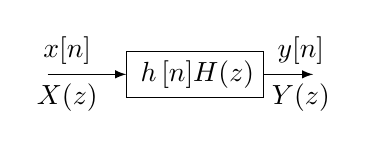
\begin{tikzpicture}
	\draw[-latex] (0,0) --++(1,0) node[near start, above] {$x[n]$} node[near start, below]  {$X(z)$} node[draw, anchor=west] (sys) {$\begin{matrix}h[n]\\H(z)\end{matrix}$};
	\draw[-latex] (sys) -- ++(1.5,0)  node[near end, above] {$y[n]$} node[near end, below]  {$Y(z)$};
\end{tikzpicture} 
    \end{center}
    \begin{align*}
        Y[n] &= h[n]\ast x[n]\\
        Y(z) &= H(z)X(z)
    \end{align*}
    \pause
    \begin{align*}
        \text{stable} &\Leftrightarrow \sum_{-\infty}^{\infty} |h[n]| < \infty\\
        \mathcal{F}\{h[n]\}&\Leftrightarrow \sum_{-\infty}^{\infty} |h[n]| < \infty\\
    \end{align*}
    \pause
    The condition for stability and the existence of the Fourier transform are the same.
\end{frame}

\begin{frame}{Stability, Causality, and ROC}
    \begin{align*}
         \text{stable} &\Leftrightarrow \text{ROC of $H(z)$ includes unit circle in $z$-plane}\\
         \text{causal} &\Rightarrow \text{$h[n]$ is right-sided}\\
         &\Rightarrow \text{ROC of $H(z)$ outside the outermost pole}\\
         \text{causal and stable} &\Leftrightarrow \text{ All poles inside unit circle}
    \end{align*}
\end{frame}

\begin{frame}{}
    \begin{example}
        Discuss the stability and causality of the system represented by the following system function with respect to different regions of convergence.
        \begin{equation*}
            H(z) = \frac{z}{\left(z-\frac{1}{3}\right)(z-2)}.
        \end{equation*}
    \end{example}
\end{frame}

\begin{frame}{}
    \begin{columns}
        \begin{column}{3in}
            \begin{center}
                \begin{tikzpicture}[scale=0.6]
    \def\pole{++(135:0.1) -- ++(-45:0.2) ++(135:0.1) -- ++(45:0.1) -- ++(-135:0.2) +(45:0.1)}
    \def\zero{circle (0.1)}
    \draw (-3, 0) -- (1,0) node[anchor=west] {$\mathrm{Re}$};
    \draw (0, -3) -- (0,3) node[anchor=south] {$\mathrm{Im}$};
    \path [pattern color=pink, pattern=north east lines] (-1, 0) ++(0,3) rectangle ++(2, -6);
    \draw (-1,0) node[anchor=north] {\scriptsize$-1$} \pole (-2, 0)  node[anchor=north] {\scriptsize$-2$} \pole;

\end{tikzpicture} 
            \end{center}
        \end{column}
        \begin{column}{2in}
            \pause
            The system is causal and unstable.
        \end{column}
    \end{columns}
\end{frame}



\begin{frame}{}
    \begin{columns}
        \begin{column}{3in}
            \begin{center}
                \usetikzlibrary{patterns}
\begin{tikzpicture}[scale=0.8]
    \def\pole{++(135:0.1) -- ++(-45:0.2) ++(135:0.1) -- ++(45:0.1) -- ++(-135:0.2) +(45:0.1)}
    \def\zero{circle (0.1)}
    	\begin{scope}
     		%\path [pattern color=pink, pattern=north east lines] (-3, -3)  rectangle (3, 3);
     		\draw [dashed, pattern color=pink, pattern=north east lines] (0,0) circle (2);
	\end{scope}

    \draw (-3, 0) -- (3,0) node[anchor=west] {\scriptsize $\mathrm{Re}$};
    \draw (0, -3) -- (0,3) node[anchor=south] {\scriptsize $\mathrm{Im}$};
    %\pause
    \draw[thick, magenta] (0,0) circle (1);
    \draw [latex-] (0,0) ++(135:1) -- ++(135:1.5) node [anchor=south east] {\scriptsize Unit circle};

    \node at (2, 1) [anchor=west] {\scriptsize $z$-plane};
    \draw (2, 0) node[anchor=north west] {$2$} \pole;
    \draw (1/3, 0) node[anchor=north ] {$\frac{1}{3}$} \pole;
	\draw    (0,0) \zero;
\end{tikzpicture} 
            \end{center}
        \end{column}
        \begin{column}{2in}
            \pause
            The system is unstable and not causal.
        \end{column}
    \end{columns}
\end{frame}

\begin{frame}{}
    \begin{columns}
        \begin{column}{3in}
            \begin{center}
                \begin{tikzpicture}[scale=0.6]
    \def\pole{++(135:0.1) -- ++(-45:0.2) ++(135:0.1) -- ++(45:0.1) -- ++(-135:0.2) +(45:0.1)}
    \def\zero{circle (0.1)}
    \draw (-3, 0) -- (1,0) node[anchor=west] {$\mathrm{Re}$};
    \draw (0, -3) -- (0,3) node[anchor=south] {$\mathrm{Im}$};
    \path [pattern color=pink, pattern=north east lines] (-1, 0) ++(0,3) rectangle ++(2, -6);
    \draw[dashed] (-2, -3) -- (-2, 3);
    \path [pattern color=orange, pattern=north west lines] (-2, 0) ++(0,3) rectangle ++(1, -6);
    \draw (-2,0) node[anchor=north] {\scriptsize$-2$} (-1,0) node[anchor=north] {\scriptsize$-1$};

\end{tikzpicture} 
            \end{center}
        \end{column}
        \begin{column}{2in}
            \pause
                The system is stable and not causal.
        \end{column}
    \end{columns}
\end{frame}





\begin{frame}
    \begin{example}
        Consider the LTI system for which the input $x[n]$ and the output $y[n]$ satisfy the linear constant-coefficient difference equation
        \begin{equation*}
            y[n] - \frac{1}{2}y[n-1] = x[n] + \frac{1}{3}x[n-1].
        \end{equation*}
        \begin{enumerate}
            \item Obtain an expression for the system function $H(z)$.
            \item What are the two choices for the region of convergence?
            \item Obtain $h[n]$ for each of these cases and comment on the stability and causality.
        \end{enumerate}
    \end{example}
    % Oppenheim p. 779
\end{frame} 